\chapter{Optimization Strategies}
\label{ch:optimization}

\fpAdd{\timegold}{0,0}{11310}
\fpAdd{\timecuda}{0,0}{1942}
\fpDiv{\speedup}{11310}{1942}

The following chapter will present optimization strategies which were used to
accelerate the mean shift image segmentation. The presented strategies are not 
onyl valid for CUDA, they can be applied to many parallel machines which are 
build after the shared memory model. 

\section{Offload Compute Intensive Parts}
\label{sec:offload_intensive}
\color{seccolor}

The amount of performance benefit an application will realize by running on CUDA
depends entirely on the extent to which it can be parallelized. As mentioned
previously, code that cannot be sufficiently parallelized should run on the
host, unless doing so would result in excessive transfers between host and
device. Amdahl’s law specifies the maximum speed-up that can be expected by
parallelizing portions of a serial program. Essentially, it states that the
maximum speed-up (S) of a program is

\begin{equation}
	S = \frac{1}{(1-p) + \frac{P}{N} }
\end{equation}

where P is the fraction of the total serial execution time taken by the portion
of code that can be parallelized and N is the number of processors over which
the parallel portion of the code runs. The larger N is (that is, the greater the
number of processors), the smaller the P/N fraction. It can be simpler to view N
as a very large number, which essentially transforms the equation into $S=1/1-P$. 
Now, if $3⁄4$ of a program is parallelized, the maximum speed-up over serial
code is $1/(1- 3/4) = 4$ . For most purposes, the key point is that the
greater P is, the greater the speed-up. An additional caveat is implicit in this
equation, which is that if P is a small number


(so not substantially parallel), increasing N does little to improve
performance. To get the largest lift, best practices suggest spending most
effort on increasing P; that is, by maximizing the amount of code that can be
parallelized.
\color{black}

The first naive implementation of the mean shift filter resulted in a speedup of
\begin{equation*}\label{eq:speedup0}
	S = \timegold\ ms/\timecuda\ ms= \speedup
\end{equation*}
times faster than the \gls{CPU} version. The reference time was
generated from
\href{http://www.caip.rutgers.edu/riul/research/code.html}{\gls{EDISON}}. It
reports timings for filtering segmentation.

\section*{Optimize Access to Global Memory}
\label{sec:coalescing}

One important fact for coalescing is the sequential accesses to global memory
should be grouped together. A simple optimization is to use the \emph{float4}
data type available in \gls{CUDA}. After rewriting the algorithm the new speedup
was 
\fpAdd{\timecuda}{0,0}{1464}
\fpDiv{\speedup}{\timegold}{\timecuda}
\begin{equation*}\label{eq:speedup0}
	S = \timegold\ ms/\timecuda\ ms = \speedup
\end{equation*}

basin of attraction, random access to global memory, not knowing where each pixel
is moving to. Switching to \emph{textures} (glossary texturess) yield to a huge
speedup of 

\fpAdd{\timecuda}{0,0}{260}
\fpDiv{\speedup}{\timegold}{\timecuda}
\begin{equation*}\label{eq:speedup0}
	S = \timegold\ ms/\timecuda\ ms = \speedup
\end{equation*}


\section*{Avoid Expensive Divisions}
\label{sec:expensive_divisions}

If possible precalculate divisions. For example if it looks like this
\begin{lstlisting}[caption=Divison, label=lst:division]
dl = (luv.x - yj_2) / sigmaR;               
du = (luv.y - yj_3) / sigmaR;               
dv = (luv.z - yj_4) / sigmaR;
\end{lstlisting}
one can calculate $rsigmaR = 1.0f/sigmaR$ in advance and everywhere where a division by
$sigmaR$ occurs replace it into a multiplication. The resulting code is
\begin{lstlisting}[caption=Precalculated Divison, label=lst:precalcdivision]
dl = (luv.x - yj_2) * rsigmaR;               
du = (luv.y - yj_3) * rsigmaR;               
dv = (luv.z - yj_4) * rsigmaR;
\end{lstlisting}

This optimization yielded  a speedup of 

\fpAdd{\timecuda}{0,0}{203}
\fpDiv{\speedup}{\timegold}{\timecuda}
\begin{equation*}\label{eq:speedup0}
	S = \timegold\ ms/\timecuda\ ms = \speedup
\end{equation*}


\section{Run Configurations} % (fold)
\label{sec:run_configurations}

It is important to check the best run configuration. Each run configruation 
has its benefit. Some can exploit the bandwidth to the global memory some can
benefit from the cache of the texture. After testing all configurations the 
best fit was a $8x32=256 threads$ configuration.

\fpAdd{\timecuda}{0,0}{181}
\fpDiv{\speedup}{\timegold}{\timecuda}
\begin{equation*}\label{eq:speedup0}
	S = \timegold\ ms/\timecuda\ ms = \speedup
\end{equation*}


% section run_configurations (end)

\section{Use the Float Data Type where Ever Possible}
One should use the $float$ data type where ever possible. \glspl{GPU} are 
highly optimized for floating point calculations. After converting all integer
calculations to floating point operations another significant speedup was 
achieved.
\fpAdd{\timecuda}{0,0}{175}
\fpDiv{\speedup}{\timegold}{\timecuda}
\begin{equation*}\label{eq:speedup0}
	S = \timegold\ ms/\timecuda\ ms = \speedup
\end{equation*}


\section{Avoid Branch Divergence} % (fold)
\label{sec:avoid_branch_divergence}
On a architecture with such high throughput of calculations per cycle it is preferred
to calculate values rather then generating them through $if$ and $else$ statements.
The remaining $if$ and $else$ statements where arranged in such a way so that a 
thread is exiting early from the loop and avoiding uneccesary calculations. This leads
of course to higher branch divergence but the execution time is lower. 
\fpAdd{\timecuda}{0,0}{125}
\fpDiv{\speedup}{\timegold}{\timecuda}
\begin{equation*}\label{eq:speedup0}
	S = \timegold\ ms/\timecuda\ ms = \speedup
\end{equation*}

\section{Shared Memory} % (fold)
\label{sec:shared_memory}
The optimization guides state that one should use shared memory to avoid 
redundant transfers from global memory. But in this case the accesses are not 
known in advance and would lead to heavy reduce in run time as the access to 
shared memory from the threads would lead to many bank conflicts. 

\section{Know the Algorithm} % (fold)
\label{sec:know_the_algo}

experiments to know how many iterations are used per pixel.... 
variying the $limit$
Setting the $lim = 10$ and executing the \gls{CPU} and \gls{GPU} version we get
\fpAdd{\tgold}{0}{7369}
\fpAdd{\tcuda}{0}{29}
\fpDiv{\speedup}{\tgold}{\tcuda}
\begin{equation*}\label{eq:speedup0}
	S = \timegold\ ms/\timecuda\ ms = \speedup
\end{equation*}


Setting the $lim = 50$ and executing the \gls{CPU} and \gls{GPU} version we get
\fpAdd{\tgold}{0}{10373}
\fpAdd{\tcuda}{0}{82}
\fpDiv{\speedup}{\tgold}{\tcuda}
\begin{equation*}\label{eq:speedup0}
	S = \timegold\ ms/\timecuda\ ms = \speedup
\end{equation*}


\begin{figure}[ht]
\centering
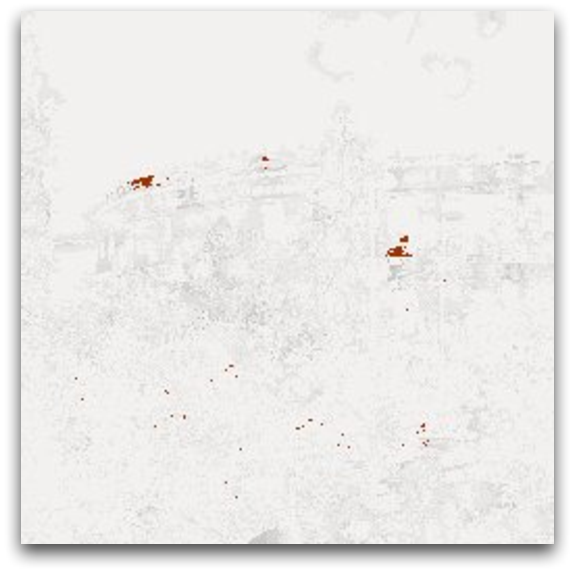
\includegraphics[width=0.6\textwidth]{gfx/itr_limitcycle0.pdf}
\caption{Visualization of Iteration Count}
\label{fig:vis_iteration_count}
\end{figure}

Looking at the iteration count  iter.txt one can see that pixel $10992$ has an 
iteration count  of $100$. 
$ i = 10992 mag=2,5 iter=100$. Examining the sequence of the magnitude one can 
easily see that after some iterations the magnitude is fixed to $2.5$. This
behaviour is known as a fixed point limit cycle.

\subsubsection{Limit Cycle, Iterating Dynamical Systems} % (fold)
\label{ssub:limit_cycle_iterating_dynamical_systems}
bla bla  limit cycle attractors...


examining $i = 15762$ shows that the iteration is a period-2 limit cycle.

Implementing a simple period-4 limit cycle detection yields to a speedup of
\fpAdd{\timecuda}{0,0}{99}
\fpDiv{\speedup}{\timegold}{\timecuda}
\begin{equation*}\label{eq:speedup0}
	S = \timegold\ ms/\timecuda\ ms = \speedup
\end{equation*}

Implementing a simple period-8 limit cycle detection yields to a speedup of
\fpAdd{\timecuda}{0,0}{87}
\fpDiv{\speedup}{\timegold}{\timecuda}
\begin{equation*}\label{eq:speedup0}
	S = \timegold\ ms/\timecuda\ ms = \speedup
\end{equation*}


\section{Unrolling Loops and Multiplications} % (fold)
\label{sec:unrolling_loops_and_multiplications}

After unrolling the multiplications 
\fpAdd{\timecuda}{0,0}{83}
\fpDiv{\speedup}{\timegold}{\timecuda}
\begin{equation*}\label{eq:speedup0}
	S = \timegold\ ms/\timecuda\ ms = \speedup
\end{equation*}

\section{Extra luv to rgb Kernel}

After a lot of optimization the most computational task became really small. Now
small function which where a tiny fraction of the complete run time became 
significant. 
After implementing a $luvtorgb$ kernel the speedup is 
\fpAdd{\timecuda}{0,0}{75}
\fpDiv{\speedup}{\timegold}{\timecuda}
\begin{equation*}\label{eq:speedup0}
	S = \timegold\ ms/\timecuda\ ms = \speedup
\end{equation*}













